\documentclass{amsart}
\usepackage[utf8]{inputenc}

\usepackage{amsthm}
\usepackage{amsmath}
\usepackage{amsfonts}
\usepackage{amssymb}
\usepackage{fullpage}
\usepackage{xcolor}
\usepackage{graphicx}
\usepackage{hyperref}
\usepackage{float}
\usepackage{algorithm}
\usepackage{algpseudocode}
\usepackage{tablefootnote}
\usepackage{caption}
\usepackage{subcaption}

\usepackage{hyperref,cleveref,color,verbatim}


\newtheorem{theorem}{Theorem}[section]
\newtheorem{prop}[theorem]{Proposition}
\newtheorem{lemma}[theorem]{Lemma}
\newtheorem{cor}[theorem]{Corollary}
\newtheorem{conj}[theorem]{Conjecture}
\newtheorem{question}[theorem]{Question}
\newtheorem{false}[theorem]{False Statement}
\newtheorem{observation}[theorem]{Observation}
\newtheorem*{theorem*}{Theorem}

\theoremstyle{definition}
\newtheorem{remark}[theorem]{Remark}
\newtheorem{defi}[theorem]{Definition}
\newtheorem{example}[theorem]{Example}

\newcommand{\fS}{\mathfrak{S}}
\newcommand{\R}{\mathbb{R}}
\newcommand{\Q}{\mathbb{Q}}
\newcommand{\C}{\mathbb{C}}
\newcommand{\EE}{\mathbb{E}}
\newcommand{\Z}{\mathbb{Z}}
\newcommand{\tr}{\textup{tr}}
\newcommand{\Ad}{\textup{Ad}}
\newcommand{\GL}{\operatorname{{\mathbf GL}}}
\newcommand{\gl}{\operatorname{gl}}
\newcommand{\FW}{\mathcal{F}\mathcal{W}}
\renewcommand{\P}{\mathcal{P}}
\newcommand{\M}{\mathcal{M}}

%%%%% debatable notations %%%%%
%%%%%%%%%%%%%%%%%%%%%%%%%%%%%%%
\newcommand\Def[1]{\emph{#1}}%
\newcommand\x{{x}}%
\newcommand\X{{X}}%
\newcommand\A{{A}}%
\newcommand\I{{I}}%
\renewcommand\a{{a}}
\renewcommand\v{{v}}%
%%%%%%%%%%%%%%%%%%%%%%%%%%%%%%%

\DeclareMathOperator*{\adj}{adj}
\DeclareMathOperator*{\Diag}{Diag}
\DeclareMathOperator*{\diag}{diag}
\DeclareMathOperator*{\Block}{B}
\DeclareMathOperator*{\Adj}{Adj}
\DeclareMathOperator*{\Span}{span}
\DeclareMathOperator*{\SO}{SO}
\DeclareMathOperator*{\supp}{supp}
\newcommand{\st}{{\text{ s.t. }}}
\newcommand{\transpose}{\intercal}
\DeclareMathOperator{\conv}{\operatorname{conv}}

\newcommand*{\Sym}{\R^{n \times n}_{\mathrm{sym}}}

\newcommand{\cL}{{\mathcal L}}
\newcommand{\De}{\operatorname{D}}
\newcommand\ks[1]{{\color{green}(Kevin: #1)}}


\DeclareMathOperator{\adju}{\operatorname{adj}}
\DeclareMathOperator{\argmin}{argmin}
\DeclareMathOperator{\argmax}{argmax}

\title{Quadratic Programs with Sparsity Constraints Via Polynomial Roots}
\date{\today}

\author{Kevin Shu}
\address[Kevin Shu]{School of Mathematics, Georgia Institute of Technology, 686 Cherry Street, Atlanta, GA 30332, USA}
\email{kshu8@gatech.edu}

\thanks{We would like to thank Greg Blekherman, Santanu Dey, and Shengding Sun for many insightful conversations. Much of the computational experiments supporting this paper were conducted at the Max Planck Institute for Mathematics in the Sciences.}

\begin{document}

\begin{abstract}
    Quadratic constrainted quadratic programs (QCQPs) are an expressive family of optimization problems that occur naturally in many applications.
    It is often of interest to seek out \emph{sparse} solutions, where many of the entries of the solution are zero.
    This paper will consider QCQPs with a single linear constraint, together with a sparsity constraint that requires that the set of nonzero entries of a solution be small.
    This problem class includes many fundamental problems of interest, such as sparse versions of linear regression and principal component analysis, which are both known to be very hard to approximate.
    We introduce a family of tractible approximations of such sparse QCQPs using the roots of polynomials which can be expressed as linear combinations of principal minors of a matrix.
    These polynomials arose naturally from the study of hyperbolic polynomials.
    Our main contributions are formulations of these approximations and computational methods for finding good solutions to a sparse QCQP.
    We will also give numerical evidence that these methods can be effective on practical problems.
\end{abstract}

\maketitle

%%%%%%%%%%%%%%%%%%%%%%%%%%%%%%%%%%%%%%%%%%%%%%%%%%%%%%%%%%%%%%%%%%%%%%%%%%%%%%%%%%%%%%%%%%%%%%
%%%%%%%%%%%%%%%%%%%%%%%%%%%INTRODUCTION&%%%%%%%%%%%%%%%%%%%%%%%%%%%%%%%%%%%%%%%%%%%%%%%%%%%
%%%%%%%%%%%%%%%%%%%%%%%%%%%%%%%%%%%%%%%%%%%%%%%%%%%%%%%%%%%%%%%%%%%%%%%%%%%%%%%%%%%%%%%%%%%%%%
\section{Introduction}
\subsection{Problem Setup}
The main objects of interest in this paper are homogeneous \emph{sparse quadratically constrainted quadratic programs} (sparse QCQPs) with a single linear constraint. Let $k$ be a nonnegative integer. A sparse QCQP is an optimization problem of the form
\begin{equation}\label{eq:sparse_qcqp_orig}
    \begin{aligned}
        \max\quad & x^{\intercal}A_0x\\
        \st & x^{\intercal}A_1x = 1\\
            & x \in \R^n\\
            &|\supp(x)| \le k.
    \end{aligned}
    \tag{$QCQP$}
\end{equation}
Here, $\supp(x) = \{i \in [n] : x_i \neq 0\}$, and $A_1, A_0 \in \Sym$.
While our techniques can produce results for sparse QCQPs with more constraints, we will focus on the one constraint case where $A_1$ is is positive definite, as it contains the problems which are of greatest interest, and also our results are especailly effective in this setting.

Two problems of this form which we will consider in detail are the \emph{sparse linear regression} and \emph{sparse maximum eigenvalue} (sparse PCA from here on) problems.
These are the natural sparse versions of the corresponding classical linear algebra problems, for which formulations as sparse QCQPs can be found in \Cref{sec:sparseReg} and \Cref{sec:sparsePCA}.
These are both problems which have been studied extensively in data science as methods for extracting features from data, for example in \cite{d2008optimal,candes2005decoding}.
Both sparse linear regression and sparse PCA are known to be NP hard \cite{welch1982algorithmic, magdon2017np}, and as such, sparse QCQPs with a single constraint in general are NP-hard to solve.

There is an extensive literature on the various types of sparse QCQPs, mostly related to the sparse linear regression and sparse PCA problems.
For this reason, and because our goal is mostly to highlight a concrete application of our algbraic methods, we will not provide an exaustive list of previous work on these subjects.
We will make particular note of approaches which increase sparsity using a penalty function such as the $\ell_1$ norm to reward solutions for being more sparse.
Such methods constitute the state of the art for sparse optimization both in theory and in practice \cite{tibshirani1996regression, hastie2020best, zou2006sparse}.
Under certain conditions, these methods can be shown to find the global optimum for \Cref{eq:sparse_qcqp_orig}, but generally, these are heuristic methods which find good solutions to the original sparse regression problem.

There have also been approaches which certify that their solutions are optimal or close to optimal, such as \cite{bertsimas2016best, bertsimas2022solving}, which use techniques such as mixed integer optimization and branch and bound.
These methods do not have polynomial time runtime, though they can be surprisingly effective on small instances of these problems.

Our method perhaps most strongly resembles greedy iterative methods for solving sparse linear regression, such as orthogonal matching pursuit \cite{tropp2004greed}.
These methods build up the support of a solution iteratively, by giving each set $T \subseteq [n]$ a score, and then adding elements to the set $T$ that maximizes the score.

Our methods are heuristic, and inspired by interior point method for solving semidefinite programs \cite{alizadeh1995interior, ben2001lectures}.
In the case of semidefinite programming, one key fact that is used for interior point methods is that the determinant function is zero on the boundary of the positive semidefinite cone.
This fact leads to a connection between the optimum value of a semidefinite program and the zero set of the determinant function.
Concretely, if we consider the one-constraint semidefinite program
\begin{equation}
    \begin{aligned}
        \max\quad & \tr(A_0X)\\
        \st & \tr(A_1X) = 1\\
            & X \succeq 0,
    \end{aligned}
\end{equation}
where $A_1$ is PSD, then the optimum value of this program is equal to the maximum zero of the univariate polynomial $g(t) = \det(A_1 t - A_0)$.
This can be seen by considering the dual semidefinite program and applying the fact that the determinant must be zero on the boundary of the PSD cone.
We will modify these facts in the sparse setting by introducing sparse versions of the determinant, and applying them to solving sparse versions of QCQPs.

We say that a polynomial $p$ in a symmetric matrix of indeterminants is a linear combination of principal minors (LPM) if it is not identically zero and it is of the form
\[
    p(X) = \sum_{S \subseteq [n] : |S| = k} a_S\det(X|_S),
\]
for some coefficients $a_S$, and where $X|_S$ denotes the principal submatrix of $X$ indexed by the set $S$.
Such polynomials were studied in \cite{blekherman2021linear} for their connection to hyperbolic polynomials and convex optimization.
In order to apply our methods, we will need as input an oracle that can efficently compute an LPM polynomial $p$ where all of the $a_S$'s are nonzero.

The key examples of such polynomials is are the \emph{characteristic coefficients}, which are supported on $\binom{[n]}{k} = \{S \subseteq [n] : |S| = k\}$:
\[
    c_n^k(X) = \sum_{S \in \binom{[n]}{k}} \det(X|_S).
\]
The characteristic coefficients are so named because they are the coefficients of the characteristic polynomial of the matrix $X$ (we will refer to \cite{horn2012matrix} for such linear algebra facts).
We will see that the characteristic coefficients have a number of properties which make it suitable for our methods, and also, it is possible to compute their values efficiently \cite{baer2021faddeev}.

Our main observation is the following: the roots of LPM polynomials can be used to bound the objective value of \Cref{eq:sparse_qcqp_orig}.
For a univariate polynomial $g(t)$, denote by $\eta_g$ the maximum real root of $g$, or $-\infty$ if $g$ has no real roots.
\begin{theorem}
    \label{thm:root_thm}
    Consider a sparse QCQP $\mathcal{Q}$ as in \Cref{eq:sparse_qcqp_orig} so that $A_1$ is positive definite.
    Suppose that $p$ is an LPM polynomial with nonnegative coefficients.
    Then there exists a feasible point $x$ to $\mathcal{Q}$ whose value is at least $\eta_g$, where $g(t) = p(A_1 t - A_0)$.

    That is, the maximum real root of the univariate polynomial $p(A_1 t - A_0)$ is a lower bound for the value of $\mathcal{Q}$.
\end{theorem}
We will discuss an alternative formulation of this theorem in terms of hyperbolic polynomials in \Cref{sec:hyperbolic}, which will allow us obtain results that relax the condition of having only 1 constraint, and also enable us to use non-positive semidefinite values for $A_1$.

We will describe how we intend to make use of this observation here.
\subsection{Contributions}
Our main contribution is to make \Cref{thm:root_thm} effective.
We provide an algorithm, \Cref{alg:greedy}, which produces solutions whose values exceed the lower bound provided in \Cref{thm:root_thm} in polynomial time.
Actually, the algorithm we propose typically finds much better solutions than what is guaranteed by the theorem.

The main idea of \Cref{alg:greedy} is to produce from a single LPM polynomial, a sequence of LPM polynomials with a decreasing number of nonzero coefficients, until in the output there is only a single nonzero coefficient.
If the final polynomial we obtain is $p = a_S \det(X|_S)$, then we output the set $S$ for the support of our final solution to \Cref{eq:sparse_qcqp_orig}.
If we can compute each of these LPM polynomials efficiently, and also, the associated root increases in each step, then we can apply \Cref{thm:root_thm} directly to see that our final solution will have objective value at least that guaranteed by \Cref{thm:root_thm}.

We also show that these roots lead to natural sparse versions of classical linear algebra theorems.
For example, in classical linear algebra, we can use Cramer's rule to show that for any matrix $A \in \R^{m\times n}$ and any $b \in \R^m$, the least squares regression loss when regressing $b$ against the columsn of $A$ is
\[
    \|b\|_2^2 - \frac{\det(A^{\intercal} ( I + bb^{\intercal})A)}{\det(A^{\intercal}A)} + 1.
\]
Similarly, for our sparse method, the upper bound on the sparse least squares regression loss guaranteed by \Cref{thm:root_thm} is given precisely by
\[
    \|b\|_2^2 - \frac{p(A^{\intercal} ( I + bb^{\intercal})A)}{p(A^{\intercal}A)} + 1.
\]
Thus, in this case, we may refer to this as a generalized Cramer's rule.

This closed form solution for this root in the case of sparse regression leads to especially efficient computational methods for this problem.
We also show that this quantity appears naturally when we consider the expectation of the least squares regression loss when regressing using a \emph{random} sample of columns of $A$ drawn from the truncated determinantal point process defined by $A^{\intercal}A$ in \Cref{sec:probabilistic}.

In the case of sparse PCA, we have the classical fact that the maximum eigenvalue of a matrix $A$ is given by
\[
    \max \{t : \det(tI - A) = 0\}.
\]
Our methods guarantee that for any LPM polynomial $p$ with nonnegative coefficients,
\[
    \max \{t : p(tI - A) = 0\}
\]
is a lower bound for the maximum $k$-sparse eigenvalue of $A$.

Once we have this effective version of \Cref{thm:root_thm}, we apply it to a few examples of interest through computational experiments.
We show in \Cref{subsec:expReg} and \Cref{subsec:expPCA} that our methods acheive results that are competitive with standard methods in such sparse optimization problems.

We also show that in principal, there is always some LPM polynomial for which \Cref{thm:root_thm} is exact in \Cref{thm:continuous_formulation}.

We conclude by describing how these methods can be generalized to multiple constraints in \Cref{sec:hyperbolic}, where we also describe the connections between these ideas and hyperbolic polynomials.

\subsection{Paper Layout}
The structure of this paper is as follows: we first describe a convex formulation of \Cref{eq:sparse_qcqp_orig} and how it naturally leads to a proof of \Cref{thm:root_thm} in \Cref{sec:lpm_relaxation}. We then define our algorithm in \Cref{subsec:heuristic} and how it specifically works for the sparse regression and sparse PCA problems in \Cref{sec:sparseReg} and \Cref{sec:sparsePCA}. We supplement this with numerical results comparing the results of these methods to state of the art methods for sparse regression. We will defer the proofs of these algorithmic results until after the experimental results, as they are of a somewhat more algebraic nature than the remainder of the paper. We conclude by describing how these results relate to the theory of hyperbolic polynomials and then some open questions.

%%%%%%%%%%%%%%%%%%%%%%%%%%%%%%%%%%%%%%%%%%%%%%%%%%%%%%%%%%%%%%%%%%%%%%%%%%%%%%%%%%%%%%%%%%%%%%
%%%%%%%%%%%%%%%%%%%%%%%%%%%LPM RELAXATIONS&%%%%%%%%%%%%%%%%%%%%%%%%%%%%%%%%%%%%%%%%%%%%%%%%%%%
%%%%%%%%%%%%%%%%%%%%%%%%%%%%%%%%%%%%%%%%%%%%%%%%%%%%%%%%%%%%%%%%%%%%%%%%%%%%%%%%%%%%%%%%%%%%%%
\section{LPM Relaxations of Sparse QCQPs}
 \label{sec:lpm_relaxation}

We will in fact consider a slightly more general problem than \Cref{eq:sparse_qcqp_orig}. Let $\Delta \subseteq 2^{[n]}$ is a family of subsets of $[n]$ where all of the elements of $\Delta$ have size $k$, then a generalized sparse QCQP is an optimization problem of the form
\begin{equation}\label{eq:sparse_qcqp}
    \begin{aligned}
        \max\quad & x^{\intercal}A_0x\\
        \st & x^{\intercal}A_1x = 1\\
            & x \in \R^n\\
            &\supp(x) \in \Delta.
    \end{aligned}
    \tag{$Q_{\Delta}$}
\end{equation}
Here, $\supp(x) = \{i \in [n] : x_i \neq 0\}$, and $A_1, A_0 \in \Sym$.

We say that an LPM polynomial $p = \sum a_S \det(X|_S)$ has support $\Delta$ if the $\{S : a_S \neq 0\} \subseteq \Delta$.

It will also be useful to think of this as a combinatorial optimization problem like so:
\begin{equation}\label{eq:sparse_qcqp_2}
    \max_{S \in \Delta}
    \begin{aligned}
        \max\quad & x^{\intercal}A_0x\\
        \st & x^{\intercal}A_1x = 1\\
            & x \in \R^S\\
    \end{aligned}
    \tag{$Q_{\Delta}$}
\end{equation}
Here, $R^S = \{x \in \R^n : \supp(x) \subseteq S\}$. The inner optimization problem can easily be solved using semidefinite programming methods for example, so the interesting question is in fact the outer optimization problem over $S$.

We now describe how the result of \Cref{thm:root_thm} arises naturally from the study of convex relaxations of \Cref{eq:sparse_qcqp}.

Various convex formulations of \Cref{eq:sparse_qcqp} have been considered, for example in \cite{atamturk2019rank, bach2010convex}.
For our purposes, we will consider the cone
\[
    \M(\Delta) = \conv \{xx^{\intercal} : x \in \R^n, \supp(x) \in \Delta\}.
\]
When $\Delta = \binom{[n]}{k}$, $\M(\Delta)$ is denoted $\FW^k_n$, and is refered to as the \emph{factor-width $k$} cone.
This cone has been studied extensively because of its connections to sparse quadratic programming \cite{boman2005factor, gouveia2022sums}.

In the one constraint case, it is not hard to see that \Cref{eq:sparse_qcqp} is equivalent to the following convex problem:
\begin{equation}
    \begin{aligned}
        \max\quad & \tr(A_0X)\\
        \st & \tr(A_1X) = 1\\
            & X \in \M(\Delta).
    \end{aligned}
    \label{eq:sparse_sdp}
\end{equation}
We think of $X$ as representing the matrix $x^{\intercal}x$, and because there is only one constraint, the optimum of this program (if it exists) must be of the form $x^{\intercal}x$ for some $x \in \R^n$ where $|\supp(x)| \le k$.

The next step in defining this heuristic is to take the dual to \Cref{eq:sparse_sdp}
\begin{equation}\label{eq:sparse_sdp_dual}
    \begin{aligned}
        \min\quad & y\\
        \st & A_1y - A_0 \in \P(\Delta).
    \end{aligned}
\end{equation}
Here,
\[
    \P(\Delta) = \{X \in \Sym : \forall S \in \Delta,\;X|_S \succeq 0\}
\] is the conical dual to $\M(\Delta)$.
When $\Delta = \binom{[n]}{k}$, this cone and its connections to hyperbolicity cones were studied extensively in \cite{blekherman2022hyperbolic}, where it was denoted by $\mathcal{S}^{n,k}$.

We will assume that strong duality holds for this problem, which in the 1-constraint setting is equivalent to saying that $-A_1$ is not in $\mathcal{P}(\Delta)$.

The main observation is that if $X \in \P(\Delta)$, and $p$ is an LPM polynomial whose coefficients are nonnegative, then $p(X) \ge 0$, simply because determinants of PSD matrices are nonnegative.
Using this observation, we may think of $\P(\Delta)$ as being a kind of barrier function for $\P(\Delta)$, in that if $p(X) < 0$, then $X$ is not in $\P(\Delta)$.
From this, we can prove \Cref{thm:root_thm} theorem easily:
\begin{proof}[Proof of \Cref{thm:root_thm}]
    Because $A_1$ is positive definite, \Cref{eq:sparse_sdp} satisfies strong duality. Therefore, we consider the dual program \Cref{eq:sparse_sdp_dual}.

    Because $A_1$ is positive definite, for $y$ large enough, $A_1 y - A_0$ will be positive definite, and in particular will be in $\mathcal{P}(\Delta)$.
    By convexity, if there is some $y_0$ so that $A_1 y_0 - A_0$ is not in $\mathcal{P}(\Delta)$ then for all $y < y_0$, $A_1 y - A_0$ is not in $\mathcal{P}(\Delta)$.

    Suppose now that $p(A_1y_0 - A_0) = 0$. Then for some $S \in \Delta$, $\det((A_1y_0 - A_0)|_S) \le 0$.
    In particular, for any $y < y_0$, $(A_1 y - A_0)|_S$ cannot be positive semidefinite.
    Therefore, we have that the value of the dual program is at least $y_0$, and by strong duality, the value of the primal program must also be at least $y_0$.
\end{proof}

This theorem actually can be extended somewhat to give a continuous optimization problem that exactly recovers the value of \Cref{eq:sparse_qcqp} (though this problem will turn out to be intractible generally).
\begin{theorem}
    \label{thm:continuous_formulation}
    Consider a sparse QCQP $\mathcal{Q}$ as in \Cref{eq:sparse_qcqp} where $A_1$ is positive definite.
    Suppose that $p$ is an LPM polynomial supported on $\Delta$ with positive coefficients. For any diagonal matrix $D$, define the polynomial
    \[
        p_D(X) = p(DXD).
    \]
    Then $p_D$ is an LPM polynomial with positive coefficients supported on $\Delta$, and the value of $\mathcal{Q}$ is precisely
    \[
        \max_{D \in \text{Diag}} \eta_{g_D},
    \]
    where $g_D = p_D(A_1t - A_0)$.
\end{theorem}
We will defer the proof of this result to \Cref{sec:continuous}.

\Cref{thm:root_thm} is the starting point for a number of results.
In \Cref{subsec:heuristic}, we will give a method for efficiently finding a feasible $x$ whose value in \Cref{eq:sparse_qcqp} matches the one guaranteed by \Cref{thm:root_thm}.
In \Cref{sec:hyperbolic}, we will also describe a way to generalize theorem \ref{thm:root_thm} to cases with multiple constraints, and when $A_1$ is not positive definite.

%%%%%%%%%%%%%%%%%%%%%%%%%%%%%%%%%%%%%%%%%%%%%%%%%%%%%%%%%%%%%%%%%%%%%%%%%%%%%%%%%%%%%%%%%%%%%%
%%%%%%%%%%%%%%%%%%%%%%%%%%%GREEDY CONDITIONING%%%%%%%%%%%%%%%%%%%%%%%%%%%%%%%%%%%%%%%%%
%%%%%%%%%%%%%%%%%%%%%%%%%%%%%%%%%%%%%%%%%%%%%%%%%%%%%%%%%%%%%%%%%%%%%%%%%%%%%%%%%%%%%%%%%%%%%%
\section{The Greedy Conditioning Heuristic}
\label{subsec:heuristic}
In this section, we give an efficient algorithm for finding a feasible $x$ to \Cref{eq:sparse_qcqp} with value at least that guaranteed by \Cref{thm:root_thm}.
We will do this using a greedy algorithm and an idea which we call the \emph{conditioning trick}.
In fact, the $x$ we will produce will often be significantly better than what is guaranteed by a naive application of \Cref{thm:root_thm}.

We will assume here that $A_1$ is positive definite for this section.

Let $p = \sum_{S \in \Delta} a_S \det(X|_S)$ be an LPM polynomial.
Given a set $T \subseteq [n]$, we define the conditional polynomial $p|_T$ to be
\[
    p|_T = \sum_{T\subseteq S \in \Delta} a_S \det(X|_S).
\]
That is, rather than summing over all $S \in \Delta$, we only sum over those $S$ in $\Delta$ that also contain $T$.

We will also extend our earlier definition of $\eta_g$ to define $\eta_{p, A_1, A_0}$ to be the maximal real root of the polynomial $p(A_1 y - A_0)$, or $-\infty$ if there is no such real root.
When $A_1$ and $A_0$ are clear from context, or implicitly defined by a sparse QCQP, we will abuse notation and simply refer to  $\eta_p$ instead of $\eta_{p, A_1, A_0}$.

Using these definitions, we can state our greedy heuristic:
we first fix an LPM polynomial with nonnegative coefficients supported on $\Delta$.
\begin{algorithm}
    \caption{The Greedy Conditioning Heuristic}
    \label{alg:greedy}
    \begin{algorithmic}
        \State $T \gets \varnothing$
        \For{$t = 1 \dots k$}
            \State $j \gets \argmax \eta_{p|_{T + j}}$
            \State $T \gets T + j$
        \EndFor

        \Return T
    \end{algorithmic}
\end{algorithm}
Intuitively, $\eta_{p|_T}$ gives us a score for how well the sets in $\Delta$ containing $T$ perform in \Cref{eq:sparse_qcqp_2}.
In each round, we add an element to our current set that maximizes the marginal improvement in this score.

\begin{theorem}
    \label{thm:greedy_works}
    Fix some LPM polynomial $p$ of degree $k$ supported on $\Delta$.
    Suppose that we have an oracle that can evaluate $p$ at any symmetric matrix $X$ in exact arithmetic.
    We can then compute $\eta_{p|_{T}}$ for any $T \subseteq [n]$ using polynomially many arithmetic operations and evaluations of $p$.
    Furthermore, \Cref{alg:greedy} produces a set $T$ so that
    \begin{equation}
        \begin{aligned}
            \max\quad & x^{\intercal}A_0x\\
            \st & x^{\intercal}A_1x = 1\\
                & x \in \R^T\\
        \end{aligned}
        \ge \eta_p.
    \end{equation}
\end{theorem}
The precise time complexity of this algorithm depends on the amount of time required to compute the values of $\eta_{p|_T}$.

In the case when $p = c_n^k$ is a characteristic coefficient, then we can bound the time complexity of this algorithm.
\begin{theorem}
    \label{thm:characteristic}
    When $p = c_n^k$, and $A_1 - A_0$ is positive definite, we can implement \Cref{alg:greedy} so that it computes a value which is at most $\eta_p + \epsilon$ using
    \[
        O(k^3(n^{\omega+1} + n\log(\frac{1}{\epsilon})))
    \]
    arithmetic operations in exact arithmetic.
\end{theorem}

In practice, numerical issues will lead to difficulties in performing these computations in exactly the way described in this document. We will discuss ways of working aroud these issues in \Cref{subsec:expReg} and \Cref{subsec:expPCA}.

%%%%%%%%%%%%%%%%%%%%%%%%%%%%%%%%%%%%%%%%%%%%%%%%%%%%%%%%%%%%%%%%%%%%%%%%%%%%%%%%%%%%%%%%%%%%%%
%%%%%%%%%%%%%%%%%%%%%%%%%%%SPARSE LINEAR REGRESSION%%%%%%%%%%%%%%%%%%%%%%%%%%%%%%%%%%%%%%%%%
%%%%%%%%%%%%%%%%%%%%%%%%%%%%%%%%%%%%%%%%%%%%%%%%%%%%%%%%%%%%%%%%%%%%%%%%%%%%%%%%%%%%%%%%%%%%%%


\section{Sparse Linear Regression}
\label{sec:sparseReg}
Given a matrix $A \in \R^{n \times m}$, $b \in \R^m$ and $k \le n$, the sparse linear regression problem is to find
\[
    \min \{ \|A x - b\|_2^2 : \|\supp(x)\| \le k\}.
\]
In \cite{ben2022new}, it was shown that this regression problem can be cast as a sparse QCQP with one constraint. In particular, this $x$ is an optimum for the sparse linear regression problem if and only if it is optimal for the following sparse QCQP:

\begin{equation*}
\begin{aligned}
    \max\quad & x^{\intercal}(A^{\intercal}bb^{\intercal}A)x\\
    \st & x^{\intercal}A^{\intercal}Ax = 1\\
        & x \in \R^n\\
        &|\supp(x)| \le k.
\end{aligned}
\label{eq:sparse_reg}
\end{equation*}
It turns out that this particular equation has a particularly simple form that allows us to find a closed form solution for the maximum root.
\begin{theorem}
    \label{thm:sparse_reg_closed_form}
    Let $p$ be an LPM polynomial with nonnegative coefficients, and suppose that $p(A^{\intercal}A) \neq 0$.
    Then for the sparse regression problem in \Cref{eq:sparse_reg}, we have that
    \[
        \eta_p = \frac{p(A^{\intercal} ( I + bb^{\intercal})A)}{p(A^{\intercal}A)} - 1.
    \]
\end{theorem}
This closed form solution bares some resemblance to Cramer's rule for finding the solution to a system of linear equations; if $p$ is the determinant, then this in fact precisely recovers Cramer's rule for solving this regression problem.recovers Cramer's rule for solving this regression problem.
It is important to note that computing this value does not require explicitly computing the roots of a polynomial; it only requires computing the value of this polynomial in two distinct points.
As a result of this, our algorithmic methods become much faster.

\begin{theorem}
    \label{thm:sparse_reg_fast}
    For sparse linear regression QCQPs, as defined in \Cref{eq:sparse_reg}, and when $p = c_n^k$, we can implement \Cref{alg:greedy} so that it requires $O(k^2n^{\omega+1})$ arithmetic operations in exact arithmetic.
\end{theorem}

\subsection{A Probabilistic Interpretation}
\label{sec:probabilistic}
We will also give a probabilistic interpretation of this value of $\eta_p$ for sparse regression.
This interpretation can be used to give intuition about when $\eta_p$ is a good approximation for sparse regression.
We take a LPM polynomial $p = \sum_{S \in \Delta} a_S \det(X|_S)$ which is supported on a set $\Delta$.
Given a matrix $A$, we consider the following probability distribution over elements of $\Delta$: we define the probability of choosing $S \in \Delta$ to be
\[
    \Pr(S) = \frac{a_S \det(A^{\intercal}A|_S)}{p(A^{\intercal}A)}
\]
If $a_S = 1$ for all $S \in \binom{[n]}{k}$, then sampling from this distribution is known as voluming sampling \cite{deshpande2006matrix}.
This is also related to the theory of determinantal point processes and strongly Rayleigh distributions \cite{anari2016monte}.
These sampling methods are often used to produce low rank sketches of a matrix; our results can be viewed as providing a deterministic method for finding such a sketch.

Intuitively, this probability distribution weights the subsets of the columns of $A$ according to their diversity; the larger the volume that that subset of columns of $A$ span, the more likely they are to be selected.
The idea of using diversity as a prior for regression was also considered in statistics, as in \cite{kojima2016determinantal}.

We also define $\ell(A_S, b) = \max \{\|b\|^2 - \|A_Sx - b\|_2^2 : x \in \R^k\}$, the squared norm of the projection of $b$ onto the column space of $A$.
\begin{theorem}
    \label{thm:probabilistic_eq}
    If $p(A^{\intercal}A) \neq 0$, then
    \[
        \eta_{p|_T} = \EE[\ell(A_S, b) | T \subseteq S].
    \]
\end{theorem}
For this reason, we think of this heuristic in this case as being a diversity weighted version of sparse linear regression.
If we think that more diverse sets of columns of $A$ will be more effective on average than less diverse sets, then this method will produce better results.
In particular, this method is not effective when the underlying matrix $A$ is essentially random, as in that case, this diversity assumption does not hold.
The case when $A$ is a Gaussian random matrix is essentially the setting of the compressed sensing problem \cite{candes2005decoding}, so in particular, this method is not especially effective for compressed sensing.

However, it seems that in real world data sets, diverse sets of columns often are preferable for regression, and so we will give experimental results for our heuristic on real world data sets in \Cref{subsec:expReg}.

%%%%%%%%%%%%%%%%%%%%%%%%%%%%%%%%%%%%%%%%%%%%%%%%%%%%%%%%%%%%%%%%%%%%%%%%%%%%%%%%%%%%%%%%%%%%%%
%%%%%%%%%%%%%%%%%%%%%%%%%%%SPARSE LINEAR REGRESSION%%%%%%%%%%%%%%%%%%%%%%%%%%%%%%%%%%%%%%%%%
%%%%%%%%%%%%%%%%%%%%%%%%%%%%%%%%%%%%%%%%%%%%%%%%%%%%%%%%%%%%%%%%%%%%%%%%%%%%%%%%%%%%%%%%%%%%%%
\section{Sparse PCA}
\label{sec:sparsePCA}
The sparse PCA problem is to find the maximum sparse eigenvector of a given symmetric matrix, or formally, for a given symmetric matrix $A$, we define the maximum $k$-sparse eigenvalue of $A$ to be the value of the following program:
\begin{equation*}
\begin{aligned}
    \max\quad & x^{\intercal}Ax\\
    \st & x^{\intercal}x = 1\\
        & x \in \R^n\\
        &|\supp(x)| \le k.
\end{aligned}
\label{eq:sparse_pca}
\end{equation*}
For a given matrix $A$, we define $\lambda^{(k)}(A)$ to be the value of this program.

\begin{lemma}
    Let $c_n^k$ be the characteristic coefficient of $X$ of degree $k$, then the
    \[
        \lambda^{(k)}(A) \ge \max \{ t : c_n^k(t I - X) = 0\} \ge \lambda_k(A),
    \]
    where $\lambda_k(A)$ is the $k^{th}$ largest eigenvalue of the matrix $A$.
\end{lemma}
The fact that $\lambda^{(k)}(A) \ge \lambda_k(A)$ has been well known, since by the Cauchy interlacing theorem, for every $S \in \binom{[n]}{k}$, $\lambda_{max}(A|_S) \ge \lambda_k(A)$.
Interestingly though, this definition also is a basis invariant property of the matrix $A$, i.e. it only depends on the eigenvalues of $A$, since the polynomial $c_n^k$ only depends on the eigenvalues of its input.

We will give experimental results for our heuristic on real world data sets in \Cref{subsec:expPCA}.

\section{Experimental Results}
In this section, we will describe our experimental results for sparse PCA and sparse linear regression.

We will exclusively use the polynomial $p = c_n^k$ for our experiments, and we will focus on the sparse linear regression problem defined in \Cref{eq:sparse_reg} and the sparse PCA problem defined in \Cref{eq:sparse_pca}.

\subsection{Some Notes on Implementation}
We implemented our methods in python using the numpy package. We ran our experiments on an 1.60GHz 4-Core Intel i5-5250u CPU with 8 GB of RAM.
Our code is available on github at \url{https://github.com/ootks/sparse_qcqps}.

In \Cref{lem:char_comp}, we described a method for computing $c_n^k$ using the Faddeev-LeVerrier method.
However, this method is numerically unstable in practice, so for our experiments, we will instead use the slower but more stable method of computing $c_n^k(X)$ by first computing the eigenvalues of $X$ and then computing the degree $k$ elementary symmetric polynomial in these eigenvalues.

Notice that \Cref{alg:greedy} is easily parallelizable, as we are computing a maximum over all elements in $[n]$ in each round, and each such computation can be done in parallel.
However, we do not do this parallelization, as our goal is primarily to demonstrate that the method performs well in terms of the final value it produces.
We expect that with further work, these methods could be made much faster, which we discuss in \Cref{sec:faster}.

\subsection{Experimental Results for Sparse Linear Regression}
\label{subsec:expReg}
In our implementation, we noticed that computing $c_n^k$ and its conditionings directly often resulted in numerical errors.
In particular, when applying \Cref{thm:sparse_reg_closed_form} to compute $\eta_{p}$, we noticed that applying it naively often resulted in subpar performance.
We mitigated this by computing $p|_T(A_1 + t A_0)$ for several values of $t$ (typically on the order of 5 values), and then using linear regression to approximate the coefficients of this linear polynomial.
We then find the root of this univariate linear polynomial.

We will evaluate our method in comparison to two existing methods, which we will describe briefly here:
\begin{itemize}
    \item LASSO\cite{tibshirani1996regression} - This minimizes the standard $L_2$ loss with an additional $L_1$ penalty added on, i.e. for some constant $\alpha$, it minimizes
    \[
        \|A x - b\|^2 + \alpha \|x\|_1.
    \]
    This is an extremely popular method for sparse linear regression.
    It is noteworthy that LASSO does not allow the user to directly specify a sparsity level, rather as $\alpha$ increases, solutions tend to become more sparse.
    Therefore, to use this as a feature selection algorithm, we first find $x$ minimizing this loss for a number of values of $\alpha$, and then we choose some threshold $\theta$ (we chose $0.09$), and let $S = \{i : x_i > \theta\}$.
    We then evaluate performance by regressing $b$ using the columns of $A$ contained in $S$ and measuring the $L_2$ loss.
    \item Orthogonal Matching Pursuit\cite{tropp2004greed} - This is an alterative greedy method for performing sparse linear regression. As in \Cref{alg:greedy}, we construct a set $S$ by adding one element in each round.
    If $T$ is the set that has been constructed so far, OMP selects the next element to maximize
    \[
        \ell(A_{T+i}, b),
    \]
    and then projects all columns of $A$ onto the orthogonal complement of the column $A_i$, and also projects $b$ onto this orthogonal complement.
\end{itemize}
We test these three methods on 4 data sets, which we refer to as \emph{Communities}, \emph{Superconductivity}, \emph{Diabetes}, and \emph{Wine}.
These datasets can all be found on the UCI Machine Learning Repository\cite{Dua:2019}, except for Diabetes, which was found in \cite{efron2004least}.

We normalize so that each column has mean 0 and variance 1.
We will evaluate both the regression loss for each method for a number of different values of $k$, and also give the time required for each method to complete.
We see from these figures that our greedy conditioning method works approximately as well as our implementation of the LASSO method in terms of regression loss, but is perhaps an order of magnitude slower.

\begin{figure}[H]
    \centering
    \textbf{Communities}\par\medskip
    \begin{subfigure}[b]{0.4\textwidth}
        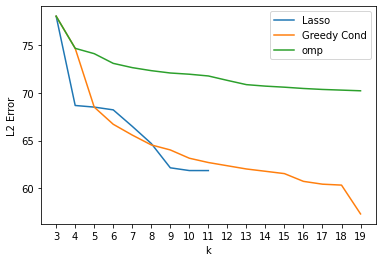
\includegraphics[width=\textwidth]{violentcrime.png}
        \caption{A plot of regression loss against $k$ for 3 methods. We could not select $\alpha$ that resulted in LASSO yielding sets of certain sizes, so they are absent from the graph.}
    \end{subfigure}
    \begin{subfigure}[b]{0.4\textwidth}
        \begin{tabular}{c c c c}
            $k$ & Greedy Conditioning & OMP & LASSO \\
            \hline
            3 & 4.11 & 0.04 & 0.04\\
            6 & 10.35 & 0.07 & 0.23\\
            9 & 15.07 & 0.11 & 0.45\\
            12 & 20.82 & 0.15 & ?\\
            15 & 28.29 & 0.18 & ?\\
            18 & 37.47 & 0.20 & ?\\
        \end{tabular}
        \vspace{0.5in}
        \caption{Selected times in seconds. For LASSO, only the run that produced a set of a given size was timed, and if no set of that size was produced, we mark it as `?'.}
    \end{subfigure}
\end{figure}
\begin{figure}[H]
    \centering
    \textbf{Superconductivity}\par\medskip
    \begin{subfigure}[b]{0.4\textwidth}
        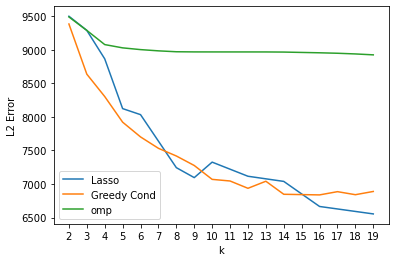
\includegraphics[width=\textwidth]{superconductivity.png}
        \caption{A plot of regression loss against $k$ for 3 methods. We could not select $\alpha$ that resulted in LASSO yielding sets of certain sizes, so they are absent from the graph.}
    \end{subfigure}
    \begin{subfigure}[b]{0.4\textwidth}
        \begin{tabular}{c c c c}
            $k$ & Greedy Conditioning & OMP & LASSO \\
            \hline
            3 & 10.11 & 0.40 & 0.08\\
            6 & 11.97 & 0.68 & 0.17\\
            9 & 13.94 & 0.97 & 0.35\\
            12 & 18.62 & 1.03 & 0.71\\
            15 & 25.97 & 1.12 & ?\\
            18 & 39.61 & 1.42 & ?\\
            \hline
        \end{tabular}
        \vspace{0.5in}
        \caption{Selected times in seconds. For LASSO, only the run that produced a set of a given size was timed, and if no set of that size was produced, we mark it as `?'.}
    \end{subfigure}
\end{figure}
\begin{figure}[H]
    \centering
    \textbf{Diabetes}\par\medskip
    \begin{subfigure}[b]{0.4\textwidth}
        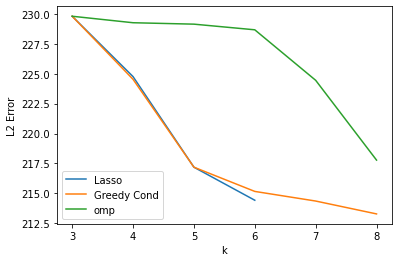
\includegraphics[width=\textwidth]{diabetes.png}
        \caption{A plot of regression loss against $k$ for 3 methods. We could not select $\alpha$ that resulted in LASSO yielding sets of certain sizes, so they are absent from the graph.}
    \end{subfigure}
    \begin{subfigure}[b]{0.4\textwidth}
        \begin{tabular}{c c c c}
            $k$ & Greedy Conditioning & OMP & LASSO \\
            \hline
            3 & 0.05 & $<10^{-2}$ & $<10^{-2}$\\
            4 & 0.05 & $<10^{-2}$ & $<10^{-2}$\\
            5 & 0.06 & $<10^{-2}$ & $<10^{-2}$\\
            6 & 0.07& $<10^{-2}$ & $<10^{-2}$\\
            7 & 0.08 & $<10^{-2}$ & ?\\
            8 & 0.09 & $<10^{-2}$ & ?\\
            \hline
        \end{tabular}
        \vspace{0.5in}
        \caption{Times in seconds. For LASSO, only the run that produced a set of a given size was timed, and if no set of that size was produced, we mark it as `?'.}
    \end{subfigure}
\end{figure}
\begin{figure}[H]
    \centering
    \textbf{Wine}\par\medskip
    \begin{subfigure}[b]{0.4\textwidth}
        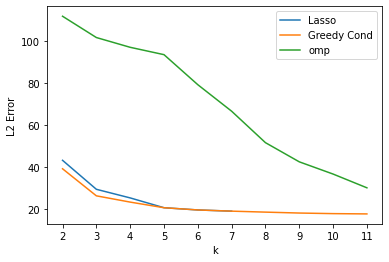
\includegraphics[width=\textwidth]{wine.png}
        \caption{A plot of regression loss against $k$ for 3 methods. We could not select $\alpha$ that resulted in LASSO yielding sets of certain sizes, so they are absent from the graph.}
    \end{subfigure}
    \begin{subfigure}[b]{0.4\textwidth}
        \begin{tabular}{c c c c}
            $k$ & Greedy Conditioning & OMP & LASSO \\
            \hline
            3 & 0.05 & $<10^{-2}$ & $<10^{-2}$\\
            6 & 0.10& $<10^{-2}$ & $<10^{-2}$\\
            9 & 0.32 & $<10^{-2}$ & ?\\
        \end{tabular}
        \vspace{0.5in}
        \caption{Times in seconds. For LASSO, only the run that produced a set of a given size was timed, and if no set of that size was produced, we mark it as `?'.}
    \end{subfigure}
\end{figure}

\subsection{Experimental Results for Sparse PCA}
\label{subsec:expPCA}
For our experimental results, we follow the work done in \cite{bertsimas2022solving}, which gives exact values for a number of real world sparse PCA problems.
We will use the optimal solutions found in their paper to benchmark our results.
We consider 5 datasets, which all come from the UC Irvine Machine Learning Repository \cite{Dua:2019}: \emph{Wine}, \emph{Pitprops}, \emph{MiniBooNE}, \emph{Communities}, and \emph{Arrythmia}.

We find that our methods produce answers which achieve close to the optimal possible answer in most cases, except where the size of the dataset is large enough that our numerical errors cause our implementation of Newton's method to fail.


\begin{table}[H]
\begin{center}
    \begin{tabular}{c|c c c c c c}
        Dataset & Columns & $k$ & Found Value & Optimal Value & Gap & Time (s)\\
        \hline
        Wine & 13 & 5 & 3.43 & 3.43 & $<10^{-6}$ & 0.30\\
             &    & 10 & 4.59 & 4.59 & $<10^{-6}$ & 1.65\\
        \hline
        Pitprops & 13 & 5 & 3.40 & 3.40 & $<10^{-5}$ & 0.24\\
             &    & 10 & 4.17 & 4.17 & $<10^{-5}$ & 1.22\\
        \hline
        MiniBooNE & 50 & 5 & 4.99 & 5.00 & $<10^{-4}$ & 3.72\\
             &    & 10 & 9.99 & 9.99 & $<10^{-4}$ & 17.96\\
        \hline
        Communities & 101 & 5 & 4.51 & 4.86 & 0.07 & 12.13 \\
             &    & 10 & 8.71 & 8.82 & $0.013$ & 686\\
        \hline
        Arrythmia & 274 & 5 & 4.18 & 4.23 & 0.012 & 173.67\\
         & & 10 & 5.73\tablefootnote{This instance was large enough that our methods suffered from numerical issues. As such, a better implementation of this method may return a better result.} & 7.53 & 0.24 & 8272
    \end{tabular}

\end{center}
\caption{A table describing the results of running an implementation of \Cref{alg:greedy} for sparse PCA on various datasets and values of $k$.  The gap is defined to be $\frac{\text{Optimal Value} - \text{Found Value}}{\text{Optimal Value}}$.}
\end{table}

%%%%%%%%%%%%%%%%%%%%%%%%%%%%%%%%%%%%%%%%%%%%%%%%%%%%%%%%%%%%%%%%%%%%%%%%%%%%%%%%%%%%%%%%%%%%%%
%%%%%%%%%%%%%%%%%%%%%%%%%%%Continuous Formulation proofs%%%%%%%%%%%%%%%%%%%%%%%%%%%%%%%%%%%%%%%%%
%%%%%%%%%%%%%%%%%%%%%%%%%%%%%%%%%%%%%%%%%%%%%%%%%%%%%%%%%%%%%%%%%%%%%%%%%%%%%%%%%%%%%%%%%%%%%%

\section{A Continuous Formulation of \Cref{eq:sparse_qcqp}}
\label{sec:continuous}
Our main goal in this section is to give a proof of \Cref{thm:continuous_formulation}
\begin{proof}%[Proof of \Cref{thm:continuous_formulation}]
    If $p$ is an LPM polynomial supported on $\Delta$ with positive coefficients, then
    \[
        p(DXD) = \sum_{S \in \Delta} \left(\prod_{i \in S} D_{ii}^2\right) a_S \det(X|_S),
    \]
    which is clearly an LPM polynomial with nonnegative coefficients.
    Therefore, by \Cref{thm:root_thm}, we have that for any $D \in \text{Diag}$, $\eta_{p_D}$ is a lower bound on the value of $\mathcal{Q}$.

    It remains to show that for some diagonal matrix $D$, we have $\eta_{p_D}$ equals the value of $\mathcal{Q}$.

    For this, let $S$ be the optimal solution in the formulation of $\mathcal{Q}$ given in \Cref{eq:sparse_qcqp_2}, and let $D$ be the diagonal matrix so that $D_{ii} = 1$ if $i \in S$, and $0$ otherwise.
    Then, we see that
    \[
        p_D(A_1 t - A_0) = a_S\det((A_1t - A_0)|_S),
    \]
    and its maximum root is precisely the value of $t$ when $(A_1t - A_0)|_S$ is PSD and singular.
    That is, this is the minimum of the program
    \begin{equation}
        \begin{aligned}
            \min\quad & y\\
            \st & (A_1y - A_0)|_S \succeq 0.
        \end{aligned}
    \end{equation}
    We see that the dual of this program is precisely
    \begin{equation}
        \begin{aligned}
            \max\quad & \tr(A_0|_SX)\\
            \st & \tr(A_1|_SX) = 1\\
                & X \succeq 0\\
        \end{aligned},
    \end{equation}
    which has precisely the value of our original program by definition of $S$.
    Moreover, strong duality holds in this case because $A_1|_S$ is positive definite, so we are done.

    We conclude that the value of $\mathcal{Q}$ is also $\eta_{p_D}$, which shows the theorem.
\end{proof}


%%%%%%%%%%%%%%%%%%%%%%%%%%%%%%%%%%%%%%%%%%%%%%%%%%%%%%%%%%%%%%%%%%%%%%%%%%%%%%%%%%%%%%%%%%%%%%
%%%%%%%%%%%%%%%%%%%%%%%%%%%greedy conditioning proofs%%%%%%%%%%%%%%%%%%%%%%%%%%%%%%%%%%%%%%%%%
%%%%%%%%%%%%%%%%%%%%%%%%%%%%%%%%%%%%%%%%%%%%%%%%%%%%%%%%%%%%%%%%%%%%%%%%%%%%%%%%%%%%%%%%%%%%%%
\section{Proofs for \Cref{subsec:heuristic} on the Greedy Conditioning Heuristic}
The goal of this section is to show that the greedy conditioning heuristic successfully finds some set $S$ which attains the value $\eta_p$ defined in \Cref{sec:lpm_relaxation}.
To do this, we will require some lemmas.
\begin{lemma}
    \label{lem:increasing}
    Assume that $A_1$ is positive definite.
    For any LPM polynomial $p$, and any $T \subseteq [n]$ so that there is some $S \in \Delta$ so that $T \subsetneq S$, there is some $i \in [n]$ so that
    \[
        \eta_{p|_{T}} \le \eta_{p|_{T + i}}.
    \]
\end{lemma}
\begin{proof}
    We have the following identity:
    \[
        (k - |T|) p|_T(X) = \sum_{i \in [n] \setminus T} p|_{T + i}(X).
    \]
    This can be seen by expanding out both polynomials in terms of minors of $X$ and comparing terms.

    Therefore, we have that $p|_T(A_1 \eta_{p|_T} - A_0) = 0 = \sum_{i \in [n] \setminus T} p|_{T + i}(A_1 \eta_{p|_T} - A_0)$.

    This implies that for some $i$, $p|_{T + i}(A_1 \eta_{p|_T} - A_0) \le 0$. Because $A_1$ is positive definite, $\lim_{t \rightarrow \infty}  p|_{T + i}(A_1 t - A_0) = \infty$, so by the intermediate value theorem, for some $t \ge \eta_{p|_T}$, $p|_{T + i}(A_1 t - A_0) = 0$, and therefore,
    \[
        \eta_{p|_{T + i}} \ge t \ge \eta_{p|_T}.
    \]
\end{proof}
\begin{lemma}
    \label{lem:new_oracle}
    Fix some LPM polynomial $p$ of degree $k$.
    Suppose that we have an oracle that can evaluate $p$ at any symmetric matrix $X$ in exact arithmetic.
    Then we can compute the value of $p|_T$ for any matrix $X$ using at most $(k+1)$ calls to the oracle and $O(n^{\omega})$ additional arithmetic operations, where $\omega$ is the matrix multiplication constant.
\end{lemma}
\begin{proof}
    To prove this, we will need to recall the Schur complement determinant identity.
    For $T \subseteq [n]$, the Schur complement of the matrix $X$ with respect to $T$ is
    \[
    X \setminus T = X|_{[n] - T} - X_{[n]-T,T} X|_T^{-1} X_{T,[n]-T},
    \]
    and we have that
    \[
    \det(X|_T) \det(X \setminus T) = \det(X).
    \]

    We also crucially have the property that Schur complements commute with taking submatrices: if $T \subseteq S$, then
    \[
    (X \setminus T)|_{S \setminus T} = (X|_S)\setminus T.
    \]
    Define $p_{-T}(X) = \sum_{S \in \Delta : T \subseteq S} a_S\det(X|_{S\setminus T})$, then from our previous lemmas,
    \[
    p|_T(X) = \det(X|_T) p_{-T}(X \setminus T).
    \]

    We can compute both $\det(X|_T)$ and $X \setminus T$ using at most $O(n^{\omega})$ arithmetic operations, so it remains to compute $ p_{-T}(X)$ using at most $k+1$ oracle calls. To do this, notice that
    \[
    \frac{\partial }{\partial X_{ii}} \det(X|_S) = \begin{cases} 0 \text{ if }i \not \in S\\ \det(X|_{S - i}) \text{ if } i \in S \end{cases}.
    \]
    From this, and extending by linearity, we get that
    \[
    p_{-T}(X) =  (\sum_{i \in T} \frac{\partial}{\partial X_{ii}})^{|T|} p|_T(X) = D_{1_{T}}^{|T|} p|_T(X).
    \]
    Here, $D_{1_{T}}$ denotes the directional derivative with respect to the diagonal matrix $1_T$ whose $i^{th}$ diagonal entry is 1 if $i \in T$ and 0 otherwise.
    We now apply an alternative characterization of the directional derivative to obtain that
    \[
    D_{1_T}^{|T|} p|_T(X) = \frac{1}{|T|!}\frac{d}{dt}^{|T|}p(X + t 1_T)|_{t = 0}
    \]
    Notice that $p(X + t 1_T)$ is a univariate polynomial of degree at most $k$, and therefore, it can be specified by its $k+1$ coefficients.
    Using our oracle, we can compute this univariate polynomial in $k+1$ distinct points.
    Using these evaluations, and we can then apply polynomial interpolation using at most $O(k^{\omega})$ additional arithmetic operations.
    Once we have the $k+1$ coefficients of $p(X+t1_T)$, we can $|T|^{th}$ derivative at 0 by just taking its $|T|^{th}$ coefficient.
\end{proof}
We come to the proof of our main theorem.
\begin{proof}[Proof of \Cref{thm:greedy_works}]
    We use \Cref{lem:new_oracle} to produce an oracle for $p|_T(X)$.
    Then, we can compute the coefficients of the polynomial $g(t) = p|_T(A_1 t - A_0)$ evaluating this polynomial at $k+1$ locations using our oracle and polynomial interpolation.
    Once we have this, we can compute $\eta|_{p|_T}$ to arbitrary accuracy using polynomial root finding techniques \cite{pinkert1976exact,ben1988fast}.

    It is clear from \Cref{lem:increasing} that at round $t$ of the algorithm,
    \[
        \eta_{p|_T} \le \max_{j \in [n] \setminus T} \eta_{p|_{T+j}}.
    \]
    In particular, we have that $\eta_{p|_T}$ increases in every round of the algorithm, and in particular, it is always at least $\eta_p$, as desired.
\end{proof}

We wish to consider a more detailed time complexity analysis when the polynomial we choose is $c_n^k$. We start with a few lemmas.
\begin{lemma}
    \label{lem:char_comp}
    Let $p = c_n^k$ be the degree $k$ characteristic coefficient of a matrix. $p|_T$ can be computed in $O(kn^{\omega})$ time.
\end{lemma}
\begin{proof}
    There are a number of ways of computing $c_n^k$. For this result, we will appeal to the well known Faddeev-LeVerrier method, which has time complexity $O(kn^{\omega})$ \cite{baer2021faddeev}. In practice, this method is incredibly numerically unstable, and so, it is often more effective to first compute the eigenvalues of $X$, and the compute the degree $k$ elementary symmetric polynomial in those eigenvalues. This requires $O(n^3)$ time.

    Once we have this oracle, the remainder of the proof procedes much as in the proof of \Cref{lem:new_oracle}, except that we note that
    \[
        p_{-T}(X) = c_n^{k-|T|}(X).
    \]
    This allows us to replace the $k+1$ oracle calls needed in the previous lemma with a single computation of $c_n^{k-|T|}(X)$.
\end{proof}

\begin{lemma}
    \label{lem:newton}
    Let $g(t)$ be a univariate polynomial with only real roots, and let $r$ be the largest root of $g(t)$.
    Then we can compute $s$ satisfying $r \le s \le r + \epsilon$ in a number of arithmetic operations which is at most
    \[
        O(k^2\log(\frac{t_0-r}{\epsilon}))
    \]
\end{lemma}
\begin{proof}
    We will consider applying the Newton iteration by taking
    \[
        x_{n+1} = x_n - \frac{g(x_n)}{g'(x_n)},
    \]
    starting at $x_1 = t_0$. Each step requires $O(k)$ arithmetic operations to compute $g$, and we wish to argue that after $k\log(\frac{g(t_0)}{\epsilon})$ steps, we will reach the largest root.

    This method is clearly shift invariant, so for the analysis, we may assume that the largest root of $g$ is at 0. We then have that
    \[
        g(t) = t(t-r_1)(t - r_2)\dots(t-r_{k-1}),
    \]
    where $r_i \le 0$ are the real roots of $g$. Therefore, $g$ has nonnegative coefficients, and we see that for $t > 0$, $g''(t) > 0$.
    Therefore, for $t > 0$, $g(t)$ is convex, and we have that
    \[
        x_n - \frac{g(x_n)}{g'(x_n)} \ge 0.
    \]
    for each $n$. Thus, this is a decreasing sequence of real numbers, which is bounded from below by 0.

    Now, using the product rule of derivatives, it can be seen that
    \[
        \frac{g(x_n)}{g'(x_n)} = \left( \frac{1}{x}+\sum_{i = 1}^{k-1} \frac{1}{x-r_i} \right)^{-1} \ge \frac{x}{k}
    \]
    Therefore,
    \[
        x_{n+1} \le \frac{k-1}{k}x_n.
    \]

    Therefore, after $k\log(\frac{t_0-r}{\epsilon})$ iterations, we will obtain that $x_{n} \le \epsilon$, as desired.
\end{proof}

\begin{proof}[Proof of \Cref{thm:characteristic}]
    We will let $p = c_n^k$.

    Firstly, note that we can compute the coefficients of the polynomial $g(t) = p|_T(A_1t - A_0)$ by first computing $g(t)$ in $k+1$ distinct points, and then applying polynomial interpolation.
    Applying \Cref{lem:char_comp}, we see that this can be done in $O(k^2n^{\omega})$ arithmetic operations.

    It follows from the work done in \cite{blekherman2021linear} that for positive definite $A_1$ and any $T$, $p|_T(A_1t - A_0)$ is real rooted.
    Moreover, from our assumption that $A_1 - A_0$ is positive definite, we obtain that the maximum root of $p|_T(A_1t + A_0)$ must lie in the interval $[0,1]$.
    We can then apply \Cref{lem:newton} using the starting point $t_0 = 1$ to obtain the maximum root to within an error of $\epsilon$ using a number of arithmetic operations bounded by
    \[
        O(k^2\log(\frac{1}{\epsilon}))
    \]

    Therefore, computing each $\eta_{p|_T}$ requires
    \[
        O(k^2(n^{\omega} + \log(\frac{1}{\epsilon})))
    \]
    arithmetic operations.

    We then must compute $\eta_{p|_T}$ $nk$ times total, so that the number of arithmetic operations is bounded from above by
    \[
        O(k^3(n^{\omega+1} + n\log(\frac{1}{\epsilon}))).
    \]
\end{proof}
\section{Proofs for \Cref{sec:sparseReg} on Sparse Linear Regression}
Our main result in this section is a proof of \Cref{thm:sparse_reg_closed_form}
\begin{proof}[Proof of \Cref{thm:sparse_reg_closed_form}]
    We consider the univariate polynomial
    \[p(A^{\intercal}A y - A^{\intercal}bb^{\intercal}A) = 0.\]

    Notice that when $y = 0$, we obtain the polynomial $p(A^{\intercal}bb^{\intercal}A)$. Now, notice that $X = A^{\intercal}bb^{\intercal}A$ is rank 1, and therefore, $\det(X|_S)$ vanishes to order $k-1$ at this point.
    Because $p$ is a linear combination of determinants, $p$ must then have a root of multiplicity at least $k-1$ at 0.

    Because $p(A^{\intercal}A) \neq 0$, and $A^{\intercal}A$ is positive semidefinite, we have that any root of this polynomial must be nonnegative, so we have that
    \[
        p(A^{\intercal}A y - A^{\intercal}bb^{\intercal}A) = y^{k-1}(ay - b) = ay^k-by^{k-1}
    \]
    for some $a,b\ge 0$. Hence, the maximal root of $p$ must be $\frac{b}{a}$.

    We can compute $a$ and $b$ explicitly. Notice that
    \[
        \lim_{y \rightarrow \infty} \frac{p(A^{\intercal}A y - A^{\intercal}bb^{\intercal}A)}{y^k} = p(A^{\intercal}A) = a,
    \]
    and that
    \[
        p(-1) = (-1)^kp(A^{\intercal}A y + A^{\intercal}bb^{\intercal}A) = (-1)^k(a+b)
    \]
    From this, we obtain that
    \[
        \frac{b}{a} = \frac{p(A^{\intercal}A y + A^{\intercal}bb^{\intercal}A)}{p(A^{\intercal}A)} - 1,
    \]
    as desired.
\end{proof}

We can apply this closed form solution to making improvements to \Cref{alg:greedy}, as in \Cref{thm:sparse_reg_fast}.
\begin{proof}[Proof of \Cref{thm:sparse_reg_fast}]
    In \Cref{alg:greedy}, the main difficulty is in computing $\eta_{p|_T}$ for $nk$ different values of $T$.

    By \Cref{thm:sparse_reg_closed_form}, we can compute $\eta_{p|_T}$ for sparse regression by evaluating $p|_T$ in two points, which is possible in time $O(kn^{\omega})$ by \Cref{lem:char_comp}.

    This implies that the final solution requires $O(k^2n^{\omega+1})$ arithmetic operations.
\end{proof}


We now show that this closed form solution is equivalent to the probabilistic result in \Cref{thm:probabilistic_eq}.
\begin{proof}[Proof of \Cref{thm:probabilistic_eq}]
    We first recall the so-called matrix determinant lemma, which states that for any invertible $X \in \R^{n\times n }$ and $v \in \R^{n}$
    \[
        \det(X + vv^{\intercal}) = (1+v^{\intercal}X^{-1}v)\det(X).
    \]

    This implies that
    \begin{align*}
        p|_{T}(A^{\intercal}A + A^{\intercal}bb^{\intercal}A) &= \sum_{S \in \Delta, T \subseteq S} a_S\det(A^{\intercal}A|_S + A^{\intercal}bb^{\intercal}A|_S)\\
                                                                   &= \sum_{S \in \Delta, T \subseteq S} a_S\det(A^{\intercal}A|_S)\big(1+b^{\intercal}A_S(A^{\intercal}A|_S)^{-1}A_S^{\intercal}b\big)\\
    \end{align*}

    We also recall the closed form formula for $\ell(A,b)$, given by
    \[
        \ell(A,b) = b^{\intercal}A(A^{\intercal}A)^{-1}A^{\intercal}b.
    \]

    We can thus simplify the above expression and see that

    \begin{align*}
        p|_{T}(A^{\intercal}A + A^{\intercal}bb^{\intercal}A) &= \sum_{S \in \Delta, T \subseteq S} a_S\det(A^{\intercal}A|_S)\big(1+\ell(A_S,b)\big)\\
                                                                   &= \left( \sum_{S \in \Delta, T \subseteq S} a_S\det(A^{\intercal}A) \right) + \sum_{S \in \Delta}\det(A^{\intercal}A|_S)\ell(A|_S,b)\\
                                                                   &= p_{\vec{a}}(A^{\intercal}A) + \sum_{S \in \Delta, T \subseteq S}a_S\det(A^{\intercal}A|_S)\ell(A_S,b)\\
    \end{align*}

    We then obtain the desired result:

    \begin{align*}
        \eta_{p|_T} = \frac{p|_{T}(A^{\intercal}A + A^{\intercal}bb^{\intercal}A)}{p|_{T}(A^{\intercal}A)} - 1 &= \big(\sum_{S \in \Delta, T \subseteq S}\Pr(S)\ell(A_S,b)\big)\\
                                                                                                      &= \EE[\ell(A_S, b) | T \subseteq S]
    \end{align*}
\end{proof}

\section{Proofs for \Cref{sec:sparsePCA} on Sparse PCA}
We show the following lemma:
\begin{lemma}
    Let $c_n^k$ be the characteristic coefficient of $X$ of degree $k$,
    \[
        \lambda^{(k)}(A) \ge \max \{ t : c_n^k(t I - X) = 0\} \ge \lambda_k(A),
    \]
    where $\lambda_k(A)$ is the $k^{th}$ largest eigenvalue of the matrix $A$.
\end{lemma}
\begin{proof}
    The first inequality follows easily from \Cref{thm:root_thm}. The inequality $\max \{ t : c_n^k(t I - X) = 0\} \ge \lambda_k(A)$ follows from root interlacing, which we will explain next.

    Let $\det(tI - X)$ be the characteristic polynomial of $X$, whose $k^{th}$ largest root is $\lambda_{k}(X)$. Then by applying the chain rule, we obtain that
    \[
        c_n^k(t I - X) = \frac{d^{n-k}}{dt^{n-k}}\det(tI - X).
    \]

    As we will discuss in the next section, the polynomial $c_n^k(tI-X)$ has only real zeros.
    Rolle's theorem implies that for a real rooted polynomial $g(t)$ with roots $r_1, \dots, r_d$, $g'(t)$ is real rooted with roots $s_1, \dots, s_{d-1}$ with the property that for $i \in [d-1]$
    \[
        r_i \le s_i \le r_{i+1}.
    \]
    See \cite{kummer2015hyperbolic} for more details.

    By induction, this implies that if the roots of $\frac{d^{n-k}}{dt^{n-k}}g(t)$ are $s_1, \dots, s_{k}$, then for $i \in [k]$,
    \[
        r_i \le s_i \le r_{n-k}.
    \]
    In this case, this implies that the largest root of $c_n^k(t I -X)$ is at least $\lambda_k(A)$.
\end{proof}
\section{Hyperbolic Polynomials}
\label{sec:hyperbolic}
We will review the theory of hyperbolic polynomials here.
An $n$-variate polynomial $p \in \R[x_1 ,\dots, x_n]$ is said to be \emph{hyperbolic} with respect to a vector $v \in \R^n$ if $p(v) > 0$ and for all $x \in \R^n$, all complex roots of the univariate polynomial $p_x(t) = p(x + tv)$ are real.
A basic example of interest for hyperbolic polynomials is the determinant of a symmetric matrix; if we take for $v$ the identity matrix $I \in \Sym$, then the spectral theorem implies that the polynomial $\det(X + tI)$ has real roots for any $X \in \Sym$.
This is equivalent to the determinant polynomial being hyperbolic with respect to the identity matrix.

Associated to any hyperbolic polynomial is its \emph{hyperbolicity cone}
\[
    \Lambda_v(p) = \{x \in \R^n : \forall t < 0, p(x + t v) \neq 0\}.
\]
Surprisingly, this set is convex for any hyperbolic polynomial. The fact that these cones are convex was first shown by G\"arding in \cite{gaarding1951linear} when studying differential equations.
Since then, hyperbolic polynomials have been studied intensely for their connections to computer science and combinatorics \cite{saunderson2019certifying, gurvits2007van, wagner2011multivariate}.

We say that a polynomial is \emph{PSD-stable} if it is defined on $\Sym$; it is hyperbolic with respect to $I$, and $\Lambda_I(p)$ contains the PSD cone.

An exact criterion for an LPM polynomial to be PSD-stable is given in \cite{blekherman2021linear}.
In particular, there exists an LPM polynomial which is PSD-stable and supported on $\Delta$ if and only if $\Delta$ is a \emph{hyperbolic matroid}, which are defined in \cite{choe2004homogeneous}.
It was also shown in \cite{blekherman2021linear} that for any PSD stable LPM polynomial supported on a set $\Delta$, $\Lambda_I(p)$ also contains $\mathcal{P}(\Delta)$.

Therefore, if we have a multivariate optimization problem of the form
\begin{equation}
    \begin{aligned}
        \min\quad & b^{\intercal} y\\
        \st & \sum_{i=1}^k A_i y_i - A_0 \in \P(\Delta),
    \end{aligned}
\end{equation}
then we can find a lower bound on this problem by considering, for any PSD-stable LPM polynomial $p$,
\begin{equation}\label{eq:sparse_lpm_dual}
    \begin{aligned}
        \min\quad & b^{\intercal} y\\
        \st & \sum_{i=1}^k A_i y_i - A_0 \in \Lambda_I(p).
    \end{aligned}
\end{equation}
This problem is tractible in the sense that $p$ serves as a self-concordant barrier function on $\Lambda_I(p)$, allowing for the usage of interior point methods to optimize as long as $p$ can be evaluated efficiently \cite{guler1997hyperbolic}.
However, there are currently no software implementations of hyperbolicity cone programming that are efficient in practice.
The main difficulty of implementing such a program at this level of generality is that $p$ usually has too many coefficients to specify precisely.

If the QCQP in question has only one constraint, then this idea allows us to extend the greedy conditioning procedure to cases when the constraint matrix $A_1$ is not positive definite.
However, even for nonsparse QCQPs with multiple constraints, it is a difficult question to understand how to recover a solution to the original QCQP from the the corresponding SDP relaxation.
It seems like it would be even harder to recover a sparse solution from our hyperbolicity cone relaxation.

For these reasons, for our main results, we only work in the 1 constraint case.

\subsection{Approximation Guarantees}
We will use the ideas contained in this section and in \cite{blekherman2022hyperbolic} to obtain some approximation guarantees for our methods.
These results will only bound the approximatation quality for $\eta_p$ for a single polynomial $p$, and thus, these results likely will not capture the quality of \Cref{alg:greedy}, which considers a large numebr of polynomials.
\begin{theorem}
    Let $\mathcal{Q}$ be a sparse QCQP with $A_1$ being positive definite with $\Delta = \binom{[n]}{k}$. Let $p = c_n^k$. Then the optimal value of $\mathcal{Q}$ is at most
    \[
        C_1\eta_{p} + C_2,
    \]
    where
    \[
        C_1 =\left(1+ \frac{(n-k)\tr(A_1)}{\lambda_{min}(A_1)n(k-1)}\right) \text{, and}
    \]
    \[
        C_2 = \frac{(n-k)\tr(A_0)}{\lambda_{min}(A_1)n(k-1)}.
    \]
\end{theorem}
\begin{proof}
    From our previous discussion, we have that
    \[
        A_1 \eta_p - A_0 \in \Lambda_I(p).
    \]
    In \cite{blekherman2022hyperbolic}, it was shown that for any $X \in \Lambda_I(p)$, $X + \frac{(n-k)\tr(X)}{n(k-1)}I \succeq 0$. Therefore,
    \[
        A_1 \eta_p - A_0 + \frac{(n-k)\tr(A_1 \eta_p + A_0)}{n(k-1)}I \succeq 0.
    \]
    Now, we have that $\frac{1}{\lambda_{min}(A_1)} A_1 \succeq I$, so we also know that
    \[
        A_1 \eta_p - A_0 + \frac{(n-k)\tr(A_1 \eta_p + A_0)}{\lambda_{min}(A_1)n(k-1)}A_1 \succeq 0.
    \]
    In particular,
    \begin{align*}
        y &= \eta_p  + \frac{(n-k)\tr(A_1 \eta_p + A_0)}{\lambda_{min}(A_1)n(k-1)}\\
         &=
        \left(1+ \frac{(n-k)\tr(A_1)}{\lambda_{min}(A_1)n(k-1)}\right)\eta_p  + \frac{(n-k)\tr(A_0)}{\lambda_{min}(A_1)n(k-1)}
    \end{align*}
    is a feasible point for \Cref{eq:sparse_sdp_dual}, and we have that $y$ is an upper bound on the optimal value of $\mathcal{Q}$.
\end{proof}
This result is somewhat crude, which is in part due to the fact that it only considers $\eta_p$, and not $\eta_{p|_T}$ for larger sets $T$.
Indeed, it can be seen that just using $\eta_p$ as a lower bound for the value of $\mathcal{Q}$ often producecs very bad results, and making use of $\eta_{p|_T}$ as in \Cref{alg:greedy} is necessary to produce interesting results.
Nevertheless, we make it explicit here as a starting point for more detailed analysis of \Cref{alg:greedy} in the future.

We can also do a crude analysis of when $\eta_p$ recovers the optimum value of \Cref{eq:sparse_qcqp_orig} exactly.
It is not hard to see from \Cref{thm:probabilistic_eq} that for sparse regression, this is only possible if, for every $S$ in the support of $p$, $S$ attains the optimum in \Cref{eq:sparse_qcqp_2}.
In fact, this is more generally true.
\begin{theorem}
    Let $p$ be a LPM polynomial with nonnegative coefficients whose support is $\Delta$.
    Let $\mathcal{Q}$ be a sparse QCQP of the form \Cref{eq:sparse_qcqp} with support $\Delta$, where $A_1$ is positive definite.
    $\eta_p$ equals the optimum value of $\mathcal{Q}$ if and only if for every $S \in \Delta$,
    \begin{equation}
    \begin{aligned}
        \max\quad & x^{\intercal}A_0x\\
        \st & x^{\intercal}A_1x = 1\\
            & x \in \R^S\\
    \end{aligned}
    \end{equation}
    equals the optimum value of $\mathcal{Q}$.
\end{theorem}
\begin{proof}
    It is the case that $\eta_p$ equals the optimum value of $\mathcal{Q}$ if and only if $\eta_p$ equals the optimum value of the dual program given in \Cref{eq:sparse_sdp_dual}.
    It can be seen that this happens if and only if
    \[
        A_1 \eta_p - A_0 \in \mathcal{P}(\Delta).
    \]
    If this occurs then we see that on the one hand, for every $S \in \Delta$,
    \[
        (A_1 \eta_p - A_0)|_S \succeq 0,
    \]
    and on the other,
    \[
        p(A_1 \eta_p - A_0) = \sum_{S \in \Delta} a_S\det((A_1 \eta_p - A_0)|_S) = 0.
    \]
    From this it follows that for all $S \in \Delta$,
    \[
        \det((A_1 \eta_p - A_0)|_S) = 0.
    \]

    Therefore, for all $S \in \Delta$, $(A_1 \eta_p - A_0)|_S$ is singular. Because $A_1$ is positive definite, we have that $\eta_p$ also solves the optimization problem
    \begin{equation}
        \begin{aligned}
            \min\quad & y\\
            \st & A_1|_Sy - A_0|_S \succeq 0.
        \end{aligned}
    \end{equation}

    We then see by strong duality that for every $S \in \Delta$,
    \begin{equation}
    \begin{aligned}
        \max\quad & x^{\intercal}A_0x\\
        \st & x^{\intercal}A_1x = 1\\
            & x \in \R^S\\
    \end{aligned}
    = \eta_p.
    \end{equation}
    This is then equal to the optimum value of $\mathcal{Q}$ by our assumption.
\end{proof}
We note that because \Cref{alg:greedy} considers a sequence of LPM polynomials, which terminates in an LPM with a singleton support, this result does not necessarily have implications for the exactness of \Cref{alg:greedy}.

\section{Conclusions and Future Directions}
Our results show that there is a fruitful connection between the roots of certain structured polynomials and sparse quadratic programming.
We have seen that these methods give an approach for a broad class of algorithmic problems, have connections to algebra, and also work well on real world optimization problems.

There are a number of ways that these results can be extended and improved.

\subsection{Different $\Delta$}
While we have seen that the set $\Delta = \binom{[n]}{k}$ has a very well behaved LPM polynomial supported on it, it is a challenge to find interesting other set families $\Delta$ for which such an LPM polynomial can be found.

Here is an example of a simple $\Delta$ which may appear in practice: say that $S_1,\dots, S_{\ell} \subseteq [n]$ are disjoint sets, and we want to ensure that at least one element from each set is chosen in our final output.
That is,
\[
    \Delta_{S_1, \dots, S_{\ell}} = \{S \subseteq [n] :|S| = k\;\forall i\in [\ell],\;S \cap S_i \neq \varnothing\}
\]
This may be of interest in practice if we have some prior information that each of these sets will contain different useful information, and so, we should take a selection from each of them.
We then define the following sequence of polynomials: we let $p_0 = c^n_k(X)$ and then define
\[
    p_i = p_{i-1}(X) - p_{i-1}(X|_{A_{i}^c}).
\]
It is not hard to see that this sequence of LPM polynomials has the desired property that it is supported exactly on $\Delta$, and that $p_{\ell}$ can be computed in time that is $O(2^{\ell}poly(n))$.
Thus, for a fixed $\ell$, this can be done efficiently, though it is unclear what to do if the number of sets grows with $n$.

In particular, we can consider a partition matroid: let $S_1, \dots, S_k$ be disjoint sets so that $S_1 \cup S_2 \cup \dots \cup S_k = [n]$ then the partition matroid for this set family is
\[
    \Delta_{S_1, \dots, S_k}  = \{S \subseteq [n] : |S \cap A_i| = 1\}.
\]
We want to understand why in the previous example, we are able to compute some associated LPM polynomial efficiently.

We define a notion of rank for a set family: the \emph{multiaffine rank} of a set family is the smallest $\ell$ so that there are diagonal matrices $D_1, \dots, D_{\ell}$ so that the LPM polynomial
\[
    \sum_{i=1}^{\ell} c_n^k(D_i X)
\]
has nonnegative coefficients and is supported on exactly $\Delta$.

It is clear that if a set family has multiaffine rank at most $\ell$, then there is an LPM polynomial supported on that set family which can be computed in $O(\ell k n^{\omega})$ time.
This is therefore an algebraic approach to understanding the complexity of computing such a polynomial.
The original example implies that for $\Delta_{S_1, \dots, S_{\ell}}$, the multiaffine rank is at most $2^{\ell}$.
We might ask if this is exactly the correct number.
\begin{question}
    What is the multiaffine rank of a partition matroid? In particular, is it $O(poly(n,k,\ell))$?
\end{question}

\subsection{Speed Improvements}
\label{sec:faster}
Our methods as they stand are significantly slower than existing methods such as LASSO for the tasks we have assigned it.
The bulk of the difficulty of running the greedy conditioning approach lies in computing the characteristic coefficients many times.
There are a few ways we can imagine improving the speed of these methods.

Simple computational improvements may be possible, but were not considered here.
For example, we may try to parallelize the computations of the characteristic coefficients in \Cref{alg:greedy}, or we may try to use better memory management at various stages.

For example, it may not be necessary to get exact results every time we compute a characterstic coefficient.
Indeed, due to numerical errors, our current methods do not exactly compute the characteristic coefficients every time.
Hence, we ask
\begin{question}
    How fast can a randomized algorithm compute the characterstic coefficient of a matrix to within an accuracy of $\epsilon$?
\end{question}

Even if it is not possible to compute a single characteristic coefficient much more quickly than what described here, the characteristic coefficients we need to compute in any given round of the algorithm are in fact all related: they are all Schur complements of a single fixed matrix. Hence, we may ask if we can acheive savings by computing all of these values simulatneously bulk.
\begin{question}
    Let $X$ be an $(n+1) \times (n+1)$ matrix. Can we compute the vector of characteristic coefficients
    \[
        (c_n^k(X \setminus 1), c_n^k(X \setminus 2), \dots, c_n^k(X \setminus n))
    \]
    in time faster than $O(kn^{\omega + 1})$?
\end{question}

It also may be possible to skip computing our $\eta_p$ heuristics for many columns of the matrix \Cref{alg:greedy}, say if on an earlier round, we see that a given column performs very poorly in comparison to other instances that have already been computed.
That is to say, if we have that in one round $\eta_{p|_{T+i}}$ is very small, on the next round, can $\eta_{p|_{T+j+i}}$ be much larger?
\begin{question}
    How much larger can $\eta_{p|_{T+i}}$ be compared to  $\eta_{p|_{T+j+i}}$ for some $j$?
\end{question}

\subsection{Approximation Guarantees}
One major aspect that is missing from our analysis is a clear theoretical understanding of which instances these methods will perform well on.
For instance, in our experiments, we see that our methods do not tend to work well on random instances.
This is not surprising in light of \Cref{sec:probabilistic}: it seems that our methods implicitly impose some prior on which subsets are more likely to perform well on these tasks.
However, our experimental results indicate that these methods should perform at least as well as LASSO in many cases.
Therefore, we may ask
\begin{question}
    What structural properties of the matrices $A_1$ and $A_0$ lead to \Cref{alg:greedy} performing close to optimally relative to the true value of \Cref{eq:sparse_qcqp}?
\end{question}
\bibliographystyle{plain}
\bibliography{biblio.bib}
\end{document}
